% Figure: Out-of-scope category — closed-world boundary inference.
% In-context KG (TQL/Cypher) underperforms NL despite full data coverage.
\begin{figure}[t]
\centering
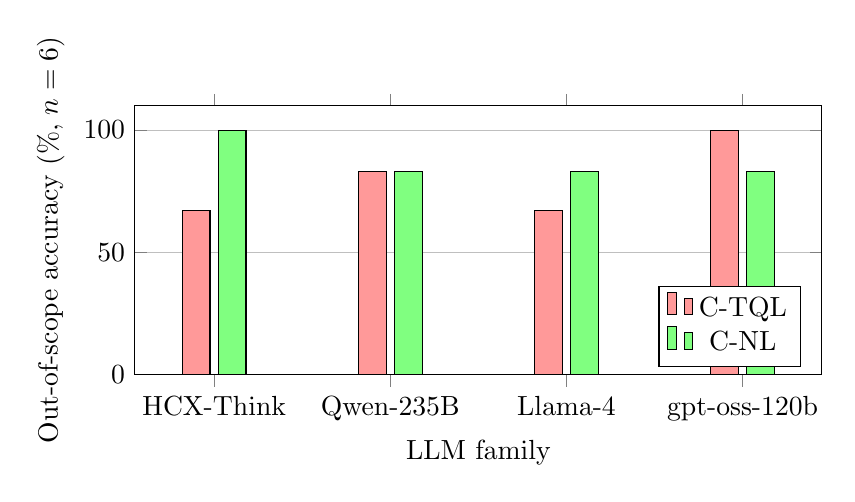
\begin{tikzpicture}
\begin{axis}[
  width=0.85\textwidth,
  height=5cm,
  ybar=3pt,
  bar width=10pt,
  ymin=0, ymax=110,
  ymajorgrids=true,
  ylabel={Out-of-scope accuracy (\%, $n=6$)},
  xlabel={LLM family},
  symbolic x coords={HCX-Think, Qwen-235B, Llama-4, gpt-oss-120b},
  xtick=data,
  legend pos=south east,
  enlarge x limits=0.15,
]
% C-TQL (formal KG)
\addplot[fill=red!40] coordinates {
  (HCX-Think, 67) (Qwen-235B, 83) (Llama-4, 67) (gpt-oss-120b, 100)
};
% C-NL (natural language)
\addplot[fill=green!50] coordinates {
  (HCX-Think, 100) (Qwen-235B, 83) (Llama-4, 83) (gpt-oss-120b, 83)
};
\legend{C-TQL, C-NL}
\end{axis}
\end{tikzpicture}
\caption{Closed-world boundary inference (out-of-scope category, $n=6$).
\textbf{Despite both surface forms containing the same facts}, the
formal KG dump (C-TQL) underperforms natural language (C-NL) on three of
four LLM families. Proving \emph{absence} requires enumeration plus
non-existence verification — a higher cognitive load that compounds with
the lower familiarity of TypeQL syntax. Sample size is small ($n=6$);
this figure is qualitative evidence; per-LLM, per-category breakdowns
are available in the released raw predictions.}
\label{fig:oos}
\end{figure}
